\subsection{m6g Family}
We now examine CPU contention on the m6g dedicated host that runs on the AWS Graviton2 
processor. It features the Nitro 2 Hypervisor, the same as the m5 family. The host has 
64 physical cores and therefore 64 vCPUs. Table \ref{tab::m6g_specs} summarizes the instance types 
belonging to this family.
\begin{table}[H]
\centering
\begin{tabular}{l|c|c}
\hline
\textbf{Instance Type} & \textbf{vCPUs} & \textbf{RAM (GiB)} \\
\hline
m6g.medium   & 1  & 4   \\
m6g.large    & 2  & 8   \\
m6g.xlarge   & 4  & 16  \\
m6g.2xlarge  & 8  & 32  \\
m6g.4xlarge  & 16 & 64  \\
m6g.8xlarge  & 32 & 128 \\
\hline
\end{tabular}
\caption{vCPU and RAM specifications for m6g instance types}
\label{tab::m6g_specs}
\end{table}
\noindent
We ran the CPU experiment across different instances types and summarized the results in 
Table \ref{tab::max_m6g}. 
\begin{table}[H]
\begin{center}
\begin{tabular}{ c|c|c|c|c|c|c }
 Instance type & medium & large & xlarge & 2xlarge & 4xlarge \\
 \hline
 Maximum Nodes & 64 & 32 & 16 & 8 & 4 \\
\hline
Degradation (Busy) \%& 0.05 & 0.03 & 0 & 0 & 0 \\
\end{tabular}
\end{center}
\caption{Maximum achievable performance degradation on our test node across various m6g instance types}
\label{tab::max_m6g}
\end{table}
\noindent 
The results show minimal degradation, which is likely caused by virtualization overhead. As 
advertised by AWS, the Nitro system causes practically no overhead (sub 0.05\%) 
and performance is almost indistinguishable from bare-metal.  
Figure \ref{fig::m6g_metal_vs_VMs} further supports this. It compares the runtime of the test node while
adding busy m5.2xlarge neighbors  to the runtime of running the threads natively on 
the m6g.metal instance. We can see that both graphs are practically similar. This behavior was
expected, since Graviton processors provide isolation between the different threads, with 
each thread running independently on a physical core. 
Graviton processors also do not support frequency scaling, so no degradation is caused by a reduction 
in average frequency. 
\begin{figure}[H]
\centering
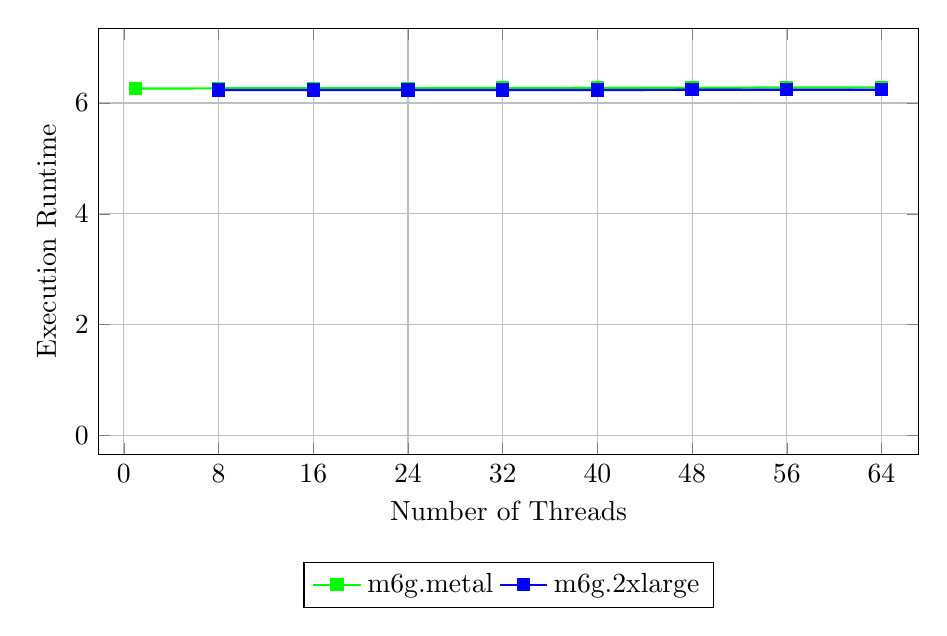
\begin{tikzpicture}
\begin{axis}[
    width=12cm,
    height=7cm,
    xlabel={Number of Threads},
    ylabel={Execution Runtime},
    grid=both,
    ymax = 7, 
    ymin = 0,
    xtick distance = 8, 
    enlargelimits=0.05,
    legend style={at={(0.5,-0.25)}, anchor=north, legend columns=2}
]

\addplot[
    color=green,
    mark=square*,
    thick
] coordinates {
    (1, 6.262)
    (8, 6.265)
    (16, 6.267)
    (24, 6.268)
    (32, 6.273)
    (40, 6.274)
    (48, 6.275)
    (56, 6.280)
    (64, 6.283)
};
\addlegendentry{m6g.metal}

\addplot[
    color=blue,
    mark=square*,
    thick
] coordinates {
    (8, 6.235)
    (16, 6.235)
    (24, 6.235)
    (32, 6.236)
    (40, 6.236)
    (48, 6.238)
    (56, 6.238)
    (64, 6.238)
};
\addlegendentry{m6g.2xlarge}


\end{axis}
\end{tikzpicture}
\caption{Effect of adding threads on the CPU performance using m6g.metal and the cpu\_burn tool}
\label{fig::m6g_metal_vs_VMs}
\end{figure}